\begin{frame}{Événements Event-B}
  \begin{itemize}
    \item<1-> Les \textbf{événements} modélisent les changements d'état du système
    \item<2-> Événements principaux dans notre modèle:
    \begin{itemize}
      \item \texttt{VehicleArrives}: Arrivée d'un véhicule dans une file
      \item \texttt{SwitchFromNS\_to\_Transition}, \texttt{SwitchFromTransition\_to\_EW}: Changements de phases
      \item \texttt{VehiclesDeparture}: Départ des véhicules aux feux verts
      \item \texttt{OptimizePhases}: Optimisation des durées de phases
    \end{itemize}
  \end{itemize}
  
  \onslide<3->{
  \begin{center}
    \begin{tikzpicture}[node distance=2cm, auto, scale=0.85]
      % Définir les styles
      \tikzstyle{phase} = [circle, draw, fill=blue!20, text width=2cm, text centered, minimum height=1cm]
      \tikzstyle{transition} = [circle, draw, fill=yellow!40, text width=2cm, text centered, minimum height=1cm]
      \tikzstyle{line} = [draw, -latex', thick]
      
      % Phases
      \node [phase] (ns) {Nord-Sud (Vert)};
      \node [transition, right=of ns] (ns_to_ew) {NS→EW (Jaune)};
      \node [phase, below=of ns_to_ew] (ew) {Est-Ouest (Vert)};
      \node [transition, left=of ew] (ew_to_ns) {EW→NS (Jaune)};
      
      % Connections
      \path [line] (ns) -- node[above] {\scriptsize SwitchFromNS\_to\_Transition} (ns_to_ew);
      \path [line] (ns_to_ew) -- node[right] {\scriptsize SwitchFromTransition\_to\_EW} (ew);
      \path [line] (ew) -- node[below] {\scriptsize SwitchFromEW\_to\_Transition} (ew_to_ns);
      \path [line] (ew_to_ns) -- node[left] {\scriptsize SwitchFromTransition\_to\_NS} (ns);
    \end{tikzpicture}
  \end{center}}
\end{frame}

\begin{frame}[fragile]{Exemple d'événement: OptimizePhases}
  \begin{lstlisting}[style=EventB]
EVENT OptimizePhases
  WHERE
    // L'événement ne peut s'exécuter que périodiquement
    timer mod OPTIMIZATION_INTERVAL = 0
  THEN
    // Ajustement des durées de phases en fonction des files d'attente
    // Actions définies de façon abstraite et raffinées dans l'implémentation
    phase_duration :| phase_duration' ∈ PHASES → ℕ
      ∧ (∀p · p ∈ PHASES ⇒ phase_duration'(p) ≥ MIN_PHASE_DURATION
                            ∧ phase_duration'(p) ≤ MAX_PHASE_DURATION)
      ∧ phase_duration'(PHASE_NS) ∝ queue_length(NORTH) + queue_length(SOUTH)
      ∧ phase_duration'(PHASE_EW) ∝ queue_length(EAST) + queue_length(WEST)
END
  \end{lstlisting}
  
  \begin{itemize}
    \item L'événement s'exécute périodiquement pour optimiser les durées
    \item Les durées sont proportionnelles aux longueurs des files d'attente
    \item Les contraintes de durées minimales et maximales sont respectées
  \end{itemize}
\end{frame}

\begin{frame}{Propriétés de sécurité vérifiées}
  \begin{columns}
    \begin{column}{0.6\textwidth}
      \begin{enumerate}
        \item<1-> \textbf{Absence de conflits:} Les feux de directions perpendiculaires ne peuvent jamais être verts simultanément
        \item<2-> \textbf{Sécurité des piétons:} Les piétons ne peuvent traverser que lorsque les véhicules correspondants sont arrêtés
        \item<3-> \textbf{Transitions sécurisées:} Les transitions entre phases incluent obligatoirement une période de feu jaune
        \item<4-> \textbf{Durées appropriées:} Les phases respectent des durées minimales et maximales
      \end{enumerate}
    \end{column}
    \begin{column}{0.4\textwidth}
      \onslide<3->{
      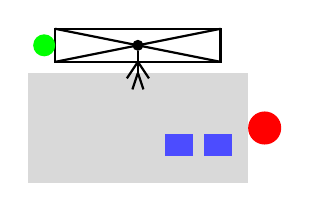
\begin{tikzpicture}[scale=0.7]
        % Route horizontale
        \fill[gray!30] (-2,0) rectangle (2,1);
        \fill[gray!30] (-2,-1) rectangle (2,0);
        
        % Feu rouge
        \fill[red] (2.3,0) circle (0.3);
        
        % Voitures en attente
        \fill[blue!70] (0.5,-0.5) rectangle (1,-0.1);
        \fill[blue!70] (1.2,-0.5) rectangle (1.7,-0.1);
        
        % Passage piéton avec personne
        \draw[thick] (-1.5,1.2) rectangle (1.5,1.8);
        \draw[thick] (-1.5,1.2) -- (1.5,1.8);
        \draw[thick] (-1.5,1.8) -- (1.5,1.2);
        
        % Figure stylisée d'un piéton
        \fill[black] (0,1.5) circle (0.1);
        \draw[thick, black] (0,1.4) -- (0,1);
        \draw[thick, black] (0,1.2) -- (-0.2,0.9);
        \draw[thick, black] (0,1.2) -- (0.2,0.9);
        \draw[thick, black] (0,1) -- (-0.1,0.7);
        \draw[thick, black] (0,1) -- (0.1,0.7);
        
        % Symbole piéton vert
        \fill[green] (-1.7,1.5) circle (0.2);
      \end{tikzpicture}}
    \end{column}
  \end{columns}
\end{frame}

\section{Algorithme d'optimisation adaptive}

\begin{frame}{Modèle mathématique d'optimisation}
  \begin{itemize}
    \item<1-> \textbf{Problématique:} Comment déterminer les durées optimales des phases?
    \item<2-> \textbf{Critère d'optimisation:} Minimiser le temps d'attente total des véhicules
    \item<3-> \textbf{Modèle adaptatif proposé:} Durées proportionnelles aux longueurs des files d'attente
  \end{itemize}
  
  \onslide<4->{
  \begin{align*}
  d_{NS} &= d_{min} + (d_{max} - d_{min}) \times \frac{q_{NS}}{q_{total}} \\
  d_{EW} &= d_{min} + (d_{max} - d_{min}) \times \frac{q_{EW}}{q_{total}}
  \end{align*}
  
  où:
  \begin{itemize}
    \item $d_{NS}$, $d_{EW}$: Durées des phases Nord-Sud et Est-Ouest
    \item $q_{NS}$, $q_{EW}$: Longueurs des files Nord-Sud et Est-Ouest
    \item $q_{total} = q_{NS} + q_{EW}$: Longueur totale des files
    \item $d_{min}$, $d_{max}$: Durées minimale et maximale des phases
  \end{itemize}}
\end{frame}

\begin{frame}{Algorithme d'optimisation adaptatif}
  \begin{algorithm}[H]
  \caption{Optimisation adaptative des durées de phases}
  $q_{NS} \gets$ longueur de la file Nord-Sud\\
  $q_{EW} \gets$ longueur de la file Est-Ouest\\
  $q_{total} \gets q_{NS} + q_{EW}$\\
  \eIf{$q_{total} > 0$}{
    $d_{NS} \gets d_{min} + (d_{max} - d_{min}) \times \frac{q_{NS}}{q_{total}}$\\
    $d_{EW} \gets d_{min} + (d_{max} - d_{min}) \times \frac{q_{EW}}{q_{total}}$
  }{
    $d_{NS} \gets d_{default}$\\
    $d_{EW} \gets d_{default}$
  }
  \end{algorithm}
  
  \begin{itemize}
    \item<2-> L'algorithme s'adapte dynamiquement aux variations du trafic
    \item<3-> Les durées restent dans des limites raisonnables: $[d_{min}, d_{max}]$
    \item<4-> En l'absence de trafic, les durées par défaut sont utilisées
  \end{itemize}
\end{frame}

\begin{frame}{Visualisation de l'optimisation}
  \begin{center}
  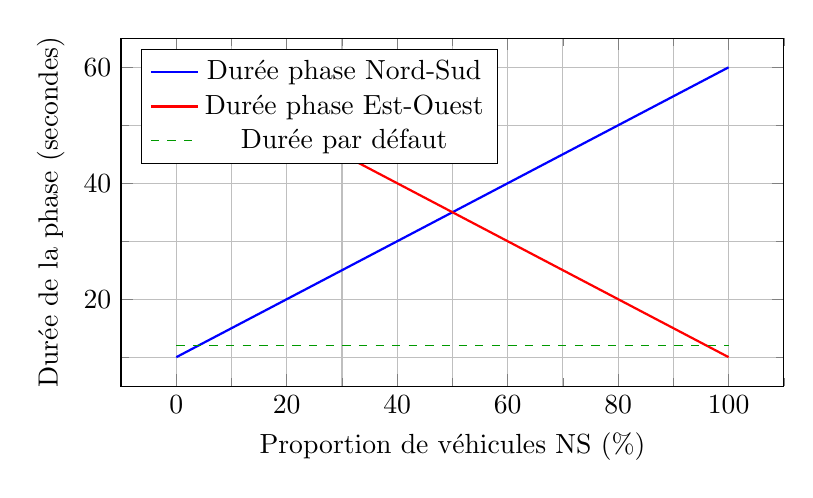
\begin{tikzpicture}
    \begin{axis}[
      width=10cm,
      height=6cm,
      grid=both,
      minor tick num=1,
      xlabel=Proportion de véhicules NS (\%),
      ylabel=Durée de la phase (secondes),
      legend pos=north west
    ]
    
    % Fonction pour la durée NS: d_min + (d_max - d_min) * (q_NS / q_total)
    \addplot[
      domain=0:100,
      samples=50,
      smooth,
      thick,
      blue,
    ] {10 + (60-10) * (x/100)};
    \addlegendentry{Durée phase Nord-Sud}
    
    % Fonction pour la durée EW: d_min + (d_max - d_min) * (q_EW / q_total)
    \addplot[
      domain=0:100,
      samples=50,
      smooth,
      thick,
      red,
    ] {10 + (60-10) * ((100-x)/100)};
    \addlegendentry{Durée phase Est-Ouest}
    
    % Ligne pour la durée par défaut
    \addplot[
      domain=0:100,
      samples=2,
      dashed,
      green!60!black,
    ] {12};
    \addlegendentry{Durée par défaut}
    
    \end{axis}
  \end{tikzpicture}
  \end{center}
  
  \begin{itemize}
    \item<2-> Lorsque le trafic NS augmente, la durée de la phase NS augmente proportionnellement
    \item<3-> Si tout le trafic est dans une direction, la durée maximale est attribuée
    \item<4-> Le modèle adaptatif assure une allocation équitable du temps
  \end{itemize}
\end{frame}
